\section{Betrachtung bestehender Lösungen}
In diesem Kapitel erfolgt eine Untersuchung des aktuellen Stands der Technik im Bereich der hardwarenahen Softwareentwicklung für Mikrocontroller.
Das Ziel besteht darin, gemeinsame Eigenschaften heraus zu arbeiten, verwendete Architekturmuster zu identifizieren und bestehende Ansätze und Konzepte zu analysieren, die das Problem der Treiberauswahl und -abstraktion lösen – insbesondere im Hinblick auf Portabilität und Wiederverwendbarkeit. 

Die Analyse dient zudem der Identifikation möglicher Lücken oder Einschränkungen bestehender Lösungen und trägt somit zur Begründung der Relevanz und Zielsetzung dieser Arbeit bei.


\subsection{Stand der Technik}
Im Rahmen der Untersuchung wurden neben Onlinerecherchen speziell zwei praxisnahe Quellen herangezogen. 
Zu den praxisnahen Quellen zählen technische Dokumentationen, Open-Source-Projekte und Herstellerdokumentationen.
Der Fokus der Recherche lag auf bestehenden Lösungen für die plattformübergreifende Auswahl von Hardwaretreibern für Mikrocontroller.
Die im Rahmen der Untersuchung verwendeten relevanten Schlüsselbegriffe umfassten unter anderem \textit{Hardware Abstraction Layer, Embedded Driver Portability, CMSIS, Arduino Core, Zephyr RTOS,C++ Hardware API Design}.

Auf diese Weise wurden verschiedene Ansätze zur Hardwareabstraktion und Treiberbereitstellung gefunden.
Die \emph{Common Microcontroller Software Interface Standard} (CMSIS)-Bibliothek ist eine von ARM entwickelte Schnittstelle, die eine weit verbreitete Anwendung findet. 
Sie bietet eine einheitliche Zugriffsebene für Cortex-M-Prozessoren. 
Herstellerbezogene Entwicklungsumgebungen wie die STM32CubeIDE von STMicroelectronics und die Espressif-IDE bieten umfangreiche Hardware-Abstraktionsbibliotheken, die gezielt auf ihre jeweiligen Mikrocontroller-Familien zugeschnitten sind.

Darüber hinaus wurden zwei Open-Source-Projekte auf GitHub analysiert: mcu-cpp und modm. 
Die Zielsetzung beider Ansätze besteht in der Modularisierung der Treiberentwicklung in C++ sowie der Bereitstellung portabler, wiederverwendbarer Hardware-APIs. 
Die Projekte zeigen eine Reihe unterschiedlicher Herangehensweisen in Bezug auf Abstraktionslevel, Architektur und Hardwareunterstützung, was wertvolle Erkenntnisse für die eigene Lösungsentwicklung bietet.
\\
\\
In den folgenden Absätzen werden die einzelnen Plattformen bewertet und potentiellen Vor- und Nachteile benannt; auch in Bezug auf die Anforderungen der eigenen Lösung. 
%Wie machen das andere; auch in Form kommerzieller Werkzeuge (cubeIDE, Espressif):
%\begin{itemize}
% 	\item CMSIS
%	\item Espressif IDE
%\end{itemize}


\subsection{STM32Cube}
Das STM32Cube-Ecosystem \cite{stm32cube_ecosystem} der Firma STMicroelectronics bietet ein gesamtes System, von der Auswahl und der Konfiguration der Hardware bis hin zu einer IDE zur Softwareentwicklung und einer Software um den internen Speicher der MCUs zu programmieren.
Die Kernprogramme sind dabei:

\paragraph{STM32CubeMX} 
	dient der Konfiguration der Hardware, d.h. Benennung und Funktionszuweisung der Pins, Aktivieren oder Deaktivieren von Registern und Protokollen, Konfiguration der internen Frequenzen über ein graphische Oberfläche.
	Nach der Konfiguration kann der Code für das Projekt generiert werden.
	In diesem Schritt werden die notwendigen Pakete, Treiber (\gls{hal}, CMSIS % TODO: CMSIS Glossareintrag
	) und Firmware für die ausgewählte Hardware geladen. \cite{stm32cubemx}

\paragraph{STM32CubeIDE}
	dient der Softwareentwicklung für die MCUs zu entwickeln und implementieren.
	Die Entwicklungsumgebung, basierend auf Eclipse, bietet neben dem Codeeditor ein eigenes Buildsystem, das mit Make und der \texttt{arm-none-ebai-gcc}-Toolchain arbeitet und einen Debugger hat, mit dem nicht nur Code sondern auch das Verhalten der Hardware beobachtet werden kann um Fehler zu erkennen. \cite{stm32cubeide}
\\
\\
Wird ein neues Projekt über STM32CubeMX gestartet werden automatisch die benötigten Hardwaretreiber und Firmware heruntergeladen und der Projektstruktur hinzugefügt, gleichzeitig wird ein Coderahmen in C generiert. 
In der Hauptheaderdatei (main.h) befinden sich neben den eingebundenen Headerdateien der Treiber auch die Pindefinitionen, die zuvor konfiguriert wurden.
In der Hauptprogrammdatei (main.c) sind generierte Funktionen für die Hardwareinitialisierung und die Pininitialisierung zu finden.
% Schichtenarchitektur
Untersucht man den Aufbau des gesamten Projekts von der Hauptdatei ausgehend soweit bis man die Register in den Funktionen der \gls{hal} findet, lassen sich Schichten erkennen.
% Anwendungsschicht
\\
\\
Allerdings ist das auch ein Aspekt, der bedacht werden muss. 
Das Softwarepaket funktioniert nur mit der STM32-Hardware.
Der Einsatz mit MCUs anderer Hersteller ist damit nicht vorgesehen.
Für allgemeine Projekte bzw. st-fremde Hardware besteht die Möglichkeit, in der STM32CubeIDE leere CMake-Projekte zu erstellen.
Hier müssen dann die benötigten Pakete und Treiber selber inkludiert werden.
Ein Buildsystem müsste selber eingebunden und mit eigenen CMake-Dateien implementiert werden.




\subsection{Espressif-IDF}
% TODO: chap4 Espressif-IDE
Aufbau / Ebenene
\begin{itemize}
	\item main
	\item Funktionen
	\item Funktionen $\rightarrow$ HAL-Funktion
	\item HAL-Funktion $\rightarrow$ LL-Funktion
	\item 
\end{itemize}


Das ESP-IDF (Espressif IoT Development Framework) stellt ein offizielles Entwicklungsframework für die Mikrocontroller der Firma Espressif dar, wie etwa das ESP32 und dessen Varianten. 
Es stellt ein umfangreiches Ökosystem bereit, das sowohl die Auswahl und Konfiguration der Hardware als auch die Entwicklung, das Flashen und Debugging von Software einschließt.

Anders als bei der STM32Cube-Umgebung gibt es hier ein primär Paket, das für die Entwicklung installiert werden muss.
Im Rahmen dieser Installation werden die erforderlichen Softwarekomponenten automatische mit integriert.
Zu diesen Komponenten zählen:

\paragraph{Toolchain}
bringt passende Compiler und die erforderlichen Werkzeuge zum Übersetzen des Quellcodes für die jeweilige ESP32-Plattform. 
Diese beinhalten die Xtensa GCC Toolchain (\texttt{xtensa-esp32-elf-gcc}) für ältere Modelle wie  ESP32-, ESP32-S2- und ESP32-S3-Modelle.
Für neuere Modelle wie den ESP32-C3 und ESP32-C6, die auf RISC-V basieren, wird die RISC-V GCC Toolchain (\texttt{riscv32-esp-elf-gcc}) verwendet.

\paragraph{Build-Tools} 
bestehen aus \texttt{CMake} und \texttt{Ninja} als Generator. 
CMake übernimmt die Konfiguration und Verwaltung des Projektes sowie die Generierung der entsprechenden Build-Files. 
Ninja sorgt für eine schnelle und effiziente Ausführung des eigentlichen Buildprozesses.

\paragraph{Python Skripte}
übernehmen Aufgaben wie die Verwaltung und Konfiguration der Entwicklungsumgebung, das Bauen von Projekten, das Flashen der Firmware auf die Zielhardware sowie die Automatisierung von häufigen Arbeitsabläufen. 
Diese Skripte verwalten im Hintergrund das Framework, sodass der Entwickler selber wenig bis garnicht mit diesen in Kontakt kommt.
Viele Befehle, wie das Kompilieren oder Hochladen, werden über diese Skripte im IDF-Terminal ausgeführt und erleichtern so die Entwicklung und den Workflow mit ESP-IDF erheblich.

\paragraph{Debug-Tools}
wie beispielsweise \texttt{OpenOCD} werden mit installiert.
Diese Werkzeuge ermöglichen neben dem Flashen der Firmware auf die Zielhardware, auch das Setzen von Breakpoints sowie das Debugging direkt auf dem Mikrocontroller. 
Sie unterstützen verschiedene Schnittstellen (z.\,B. JTAG oder USB) und lassen sich mit gängigen IDEs und Entwicklungsumgebungen integrieren.


Wird ein neues Projekt mit dem ESP-IDF Framework gestartet, erfolgt die Einrichtung der Projektstruktur und der benötigten Komponenten ebenfalls weitgehend automatisiert.
Die Generierung eines neuen Projekts kann über die Kommandozeile des IDF-Terminal oder entsprechende Assistenten wie der ESP-IDF Erweiterung in VSCode erfolgen.
In diesem Prozess generiert das Framework die zugehörige Ordnerstruktur, den Beispielcode sowie die Konfigurationsdateien.
Die erforderlichen Hardwaretreiber, Bibliotheken und Tools wurden bereits mit der Installation des Frameworks bereitgestellt, sodass ein weiterer Download nicht mehr notwendig ist.














































% TODO: chap4 mcu-cpp & modm: Tiefer Analyse: Wie ist der Code aufgebaut -> Architektur-Muster

\subsubsection{mcu-cpp}
Das Open-Source-Projekt \emph{mcu-cpp} verwendet einen eigenen \texttt{namespace} um die einzelnen Funktionen und Klassen zu gruppieren.
\emph{Namespaces} sind eine Möglichkeit in C++ um Variablen, Klasse und Funktionen zu gruppieren, damit Konflikte bei der Benennung solcher Identifizierer zu vermeiden.
Dies ermöglicht es einen sauber-strukturierten und lesbaren Applikationscode zu schreiben, in dem man nachvollziehen kann, wer was aufruft.
Basierend auf den virtuellen Klassen, werden die jeweiligen Methoden von den \gls{mcu}s implementiert.
Um innerhalb einer Produktfamilie, z.B. STM32F0 MCUs, die richtigen bzw. alle notwendigen Ports zu aktivieren, gibt es eine zusätzliche Datei \texttt{gpio\_hw\_mapping.hpp}.
In dieser werden einzelne Ports, die nicht auf jeder MCU verfügbar sind, durch bedingte Kompilierung aktiviert oder nicht.
Die Information, welche Hardware verwendet wird, muss entweder in der \texttt{CMakeLists.txt} oder im Code mit \texttt{\#define} angegeben sein.
Zusätzlich werden die CMSIS-Treiber verwendet, die die Startdateien bereit stellen.
Als RTOS ist FreeRTOS fest im Projekt integriert.
%Dies ermöglicht
Allerdings fehlen hier die offiziellen \emph{Hardware-Abstracition-Layer} (HAL) Funktionen, die bereits vorgefertigte Strukturen und Funktionen für die einzeln Hardwarefunktionen implementiert haben.
Stattdessen werden diese durch die Implementierung der virtuellen Klassen ersetzt.
Das sorgt im weiteren Verlauf dafür, dass die Funktionen auf Basis der virtuellen Klassen für jede neue MCU-Familie neu implementiert werden muss, was einen für wiederholten Aufwand sorgt und den Anforderungen an die Lösung widerspricht.

Untersucht man das Projekt auf Architektur- und Designmuster lassen sich die gleichen Muster identifizieren wie bei den STM32-Projekten.
Es wird in einer Schichtenarchitektur gearbeitet.
Die Aufteilung ist nahezu identisch, mit dem Hauptprogramm in der Anwendungsschicht, der Hardwareabstraktion mit den CMSIS Dateien und neu geschriebenen Abstraktionsfunktionen, statt den klassischen \gls{hal}-Bibliothek.
Mit der Verwendung von FreeRTOS kommt die Middleware-Schicht, die sich zwischen der Anwendungsschicht und der Abstraktionsschicht befindet.
% Design
Designmuster ähneln sich ebenfalls.
Für die Hardwareinitialisierung wird das Singleton verwendet.
Es gibt nur eine globale Instanz der \texttt{systick}-Klasse.
Darüber hinaus gibt es keine erkennbaren Erzeugungsmuster.
Die Auswahl der Hardware findet über die Haupt-\texttt{CMakelists.txt}-Datei statt.

Im Bereich der Strukturmuster lässt sich das Facade-Pattern erkennen.
Beispielsweise dient die Klasse gpio\_stm32f4 der Abstraktion der Initialisierung und Steuerung von GPIOs über Registeroperationen in eine klar strukturierte, objektorientierte Schnittstelle. 
Für Entwickler besteht somit die Möglichkeit, GPIOs einfach per Konstruktor und Methoden wie \texttt{set()}, \texttt{toggle()}, \texttt{mode()} oder \texttt{get()} zu verwenden, ohne sich mit den zugrunde liegenden Bitmanipulationen und der Clock-Konfiguration befassen zu müssen. 

Im Bereich der Verhaltensmuster finden sich mehrere Beispiele:

Das Template Method Pattern findet in der \texttt{systick}-Komponente Anwendung. 
Der Ablauf der Interruptbehandlung ist in der entsprechenden Stelle explizit definiert, ermöglicht jedoch die Integration individueller Erweiterungspunkte (beispielsweise durch überschreibbare oder registrierbare Callbacks wie \texttt{onTick()}). 
Diese Erweiterungspunkte können angepasst werden, ohne dabei den Ablauf der Interruptbehandlung selbst zu modifizieren.

Ein weiteres Verhaltensmuster ist das Observer Pattern, das bei der Behandlung von GPIO-Interrupts zum Einsatz kommt.
Die Anwendung ist in der Lage, über Callbacks oder Eventhandler auf externe Ereignisse zu reagieren, die von der Peripherie ausgelöst und vom ISR (Interrupt Service Routine) weitergeleitet werden. 
Hieraus resultiert ein charakteristisches Beobachterverhältnis zwischen Hardwareereignis und Anwendungslogik.

Darüber hinaus lässt sich ein Strategy-Pattern in der SPI-Implementierung identifizieren, bei dem zur Compile- oder Laufzeit unterschiedliche DMA-Komponenten eingebunden werden können. 
Das Verhalten der Datenübertragung unterliegt einer dynamischen Veränderung durch den Austausch von Komponenten.

% TODO: chap4 mcu-cpp: Quellen-Verlinkung
Das Open-Source-Projekt \emph{mcu-cpp} verwendet einen eigenen \texttt{namespace} um die einzelnen Funktionen und Klassen zu gruppieren.
\emph{Namespaces} sind eine Möglichkeit in C++ um Variablen, Klasse und Funktionen zu gruppieren, damit Konflikte bei der Benennung solcher Identifizierer zu vermeiden.
Die ermöglicht einen sauber-strukturierten und lesbaren Applikationscode zu schreiben, in dem man nachvollziehen kann, wer was aufruft.
Basierend auf den virtuellen Klassen, implementieren die jeweiligen MCUs die Methoden damit diese für sich funktionieren.
Um innerhalb einer Produktfamilie, z.B. STM32F0 MCUs, die richtigen bzw. alle notwendigen Ports zu aktivieren, gibt es eine zusätzliche Datei \texttt{gpio\_hw\_mapping.hpp}.
In dieser werden einzelne Ports, die nicht auf jeder MCU verfügbar sind, durch bedingte Kompilierung aktiviert oder nicht.
Die Information, welche Hardware verwendet wird, muss entweder in der \texttt{CMakeLists.txt} oder im Code mit \texttt{\#define} angegeben sein.
Zusätzlich werden die CMSIS-Treiber verwendet, die die Startdateien bereit stellen.
Als RTOS wird aktuell FreeRTOS verwendet.
%Dies ermöglicht
Allerdings fehlen hier die offizielle \emph{Hardware-Abstracition-Layer} (HAL), die bereits vorgefertigte Strukturen und Funktionen für die einzeln Hardwarefunktionen implementiert haben.
Stattdessen werden diese durch die Implementierung der virtuellen Klassen ersetzt.
Das sorgt im weiteren Verlauf dafür, dass die Funktionen auf Basis der virtuellen Klassen für jede neue MCU-Familie neu implementiert werden muss, was einen für wiederholten Aufwand sorgt und den Anforderungen an die Lösung widerspricht.



\subsubsection{modm}
% TODO: chap4 modm: Quellen-Verlinkungß
Das Open-Source-Projekt \emph{modm} dient als Baukasten um zugeschnittene und anpassbare Bibliotheken für Mikrocontroller zu generieren.
Dadurch ist es möglich, dass eine Bibliothek nur aus den Teilen besteht, die tatsächlich in der Applikation und im Code verwendet werden müssen, ohne das es einen unnötig großen Overhead gibt.
Um das zu bewerkstelligen wird eine Kombination aus \texttt{Jinja2}-Template-Dateien, \texttt{lbuild}-Pyhton-Skripte und eigenen Moduldefinitionen verwendet, mit der der Code für die Bibliotheken generiert wird.
Die Templatedateien enthalten Platzhalter.
Die Werte kommen aus \texttt{YAML} und \texttt{JSON}-Dateien, die von den \texttt{lbuild}-Pyhtonskripten gelesen und in die entsprechenden Positionen der Platzhalter, während des Buildprozesses, eingefügt werden.
 
Um eine Bibliothek zu erstellen, muss ein Prozess über die Konsole gestartet werden.
modm hat bereits vordefinierten Konfigurationen für eine große Auswahl an MCUs.
Mit diesen kann die Bibliothek für ein Projekt erstellt werden.

Will man aber Module verwenden, die in der vordefinierten Konfiguration nicht enthalt sind, kann man diese einzeln zu der \texttt{project.xml} hinzufügen.
Um sehen zu können welche Module zur Verfügung stehen muss folgende Zeile in der Konsole ausgeführt werden:

\vspace{3mm}
\begin{lstlisting}[language=bash, caption={Konsolenbefehl um verf\"ugbare Module aufgelistet zu bekommen; hier f\"ur den STM32C031C6T6 Mikrokontroller.}, label={lst:modm_lbild_discover}]
\modm\app\project>
	lbuild --option modm:target=stm32c031c6t6 discover
\end{lstlisting}

Sobald die gewünschten Module hinzugefügt wurde, beginnt der Installations- bzw. der Generierungsprozess der Library. 
Gibt man nun \texttt{lbuild builld} in der Konsole ein wenn man sich im \texttt{app/project}-Verzeichnis befindet, kann die Bibliothek erstellt werden.
Nach erfolgreichem Build erscheint in dem Projektverzeichnis ein neuer Ordner \emph{modm}.
Dieser enthält die generierten Dateien der ausgewählten Module.

%Positiv hervorzuheben ist hier das (vordergründige) simple Hinzufügen von Modulen.
%Da das Projekt aktuell bereits sehr umfangreich ist und sehr viele Mikrokontroller und Optionen unterstützt, bietet es eine große Auswahl an Modulen, die beliebig zu einem Projekt hinzugefügt werden können.
%
%Allerdings ist zu beachten, dass falls man zukünftig neue Module oder Mikrokontroller hinzufügen will, müssen diese an die bestehende Struktur angepasst und in das Zusammenspiel von Python, Jinja2 und den YAML/JSON-Dateien integriert werden.
%Dies ist mit einem sehr hohen Aufwand verbunden.

% Architektur
Wird ein Projekt erstellt, dass eine generierte modm-Bibliothek verwendet, lassen sich auch hier bereits bekannte Muster, wie die Schichtenarchitektur, erkennen.
Anwendungs- und Middlewareschicht unterscheiden sich im Inhalt nicht von dem bereits bekannten aus mcu-cpp und STM32CubeIDE.
Die Anwendungsschicht enthält weiterhin die Hauptdatei, die Businesslogik und eigene erstellt Klassen, die die Funktionen der tieferliegenden Schichten verwenden.
Die Middlewareschicht ist weiterhin optional.
Wurde im Konfigurationsprozess der Bibliothek keine \gls{rtos} oder keine erweiternden Funktionen wie USB und Netzwerkanbindung ausgewählt, sind diese im Projekt ebenfalls nicht vorhanden.
Unterschiede sind in der Abstraktionsschicht zu finden.
Diese verwendet keine bereits vorhandenen Funktionen oder Bibliotheken wie die STM32-\gls{hal}, sondern wird vollständig durch modm generiert.
Sie besteht u.a. aus der Datei \texttt{board.hpp}, die typsichere GPIO-Definitionen, Peripherieklassen (z.B. für SPI und ADC) sowie Funktionen zur Initialisierung und Konfiguration enthält; ähnlich der \texttt{main.h} eines STM32Cube-Projektes.
Dadurch erfolgt eine Kapselung des direkten Zugriffs auf Hardware sowie die Bereitstellung einer objektorientierten API.
Die unterhalb liegende Hardwareschicht besteht aus templatespezifischen Registerzugriffen. 
Funktionen wie \texttt{GpioA0::setOutput()} ermöglichen den direkten Zugriff auf die Register. 
Der Einsatz dieser Low-Level-Operationen erfolgt ausschließlich über die Abstraktionsschicht.
% Designmuster
Im modm-Projekt findet bewusst auf die Verwendung klassischer Designmuster in ihrer typischen objektorientierten Form, verzichtet. 
Stattdessen werden zahlreiche Funktionalitäten durch statische Metaprogrammierung, Templates und generische Programmierung abgebildet. 
Nichtsdestotrotz lassen sich in der Struktur und Verwendung bestimmter Klassen Parallelen zu bekannten Entwurfsmustern erkennen.
%Erzeugungmuster
Ähnlich dem Singleton-Pattern, kann bei einer Vielzahl von GPIO-Objekten und Board-Komponenten, wie beispielsweise \texttt{Board::LedD13} oder \texttt{Board::PushButton}, ein vergleichbare Aufbau beobachten werden.
So ist es möglich, die betreffenden Elemente über statische Typen eindeutig zu referenzieren. 
Dadurch wird eine einzige, globale Instanz je Pin bereitgestellt.

Die Initialisierung über \texttt{Board::initialize()} oder die vordefinierten Aliase wie \texttt{Board::LedD13} können als eine Art Factory betrachtet werden. 
Dies liegt an einer einheitlichen, zentralisierten Bereitstellung von Komponenten für die Anwendung.
Eine echte Factory-Methode im GoF-Sinn ist jedoch nicht implementiert, da keine polymorphe Objekterzeugung zur Laufzeit stattfindet.

Mit Blick auf Strukturmuster können Ähnlichkeiten zum Composite Muster gezogen werden.
Strukturen wie \texttt{GpioSet<GpioA0, GpioA1, GpioA2>} fungieren hierbei als logische Zusammenfassung mehrerer GPIOs.
Obwohl keine echte rekursive Baumstruktur mit abstrakter Basisklasse, wie sie im klassischen Composite Pattern vorliegt, ähneln solche Klassen diesem Muster insofern, als dass sie gemeinsame Operationen, z. B. \texttt{set()}, \texttt{reset()}, auf eine gesamte Gruppe anwenden. 

Ein Verhaltensmuster wie es zuvor in mcu-cpp und STM32Cube-Projekt vorhanden war, ist hier nicht zu erkennen.

Insgesamt fokussiert sich das modm-Projekt auf eine compilezeit-optimierte Architektur, durch die klassische Entwurfsmuster nur begrenzt bzw. in abgewandelter Form eingesetzt werden.
























































%\vspace{3mm}
%\begin{figure}[H]
%	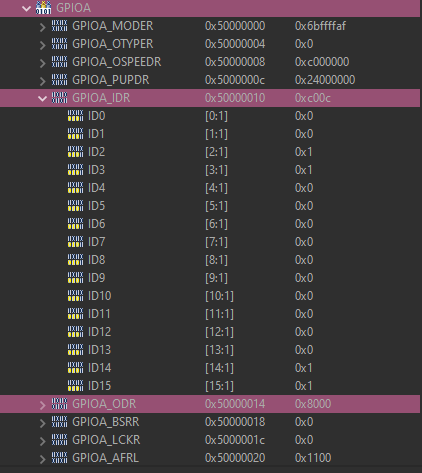
\includegraphics[width=\textwidth]{stm32_c031c6_clean_registers_setPin.PNG}
%	\caption{Register beim setzen des Pin.}
%	\label{fig:stm32_register_setPin}
%\end{figure}
%
%\vspace{3mm}
%\begin{figure}[H]
%	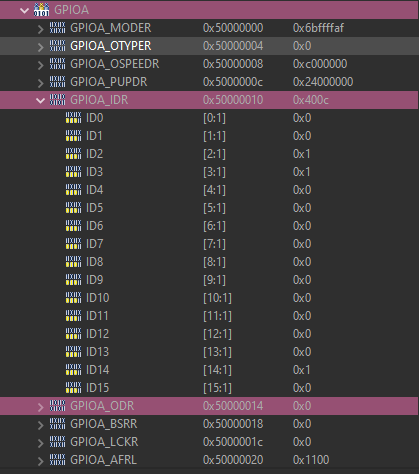
\includegraphics[width=\textwidth]{stm32_c031c6_clean_registers_resetPin.PNG}
%	\caption{Register beim zurücksetzen des Pin.}
%	\label{fig:stm32_register_resetPin}
%\end{figure}
%
%In den Abbildungen \autoref{fig:stm32_register_setPin} und \autoref{fig:stm32_register_resetPin} ist der Wert von Pin 15 (ID15 \& OD15) zu beobachten. Bei \texttt{0x0} wird der Pin zurückgesetzt und die LED leuchtet nicht mehr. Bei \texttt{0x1} wird der Wert auf $1$ gesetzt und die LED beginnt zu leuchten.
%
%Die Funktionen \texttt{HAL\_GPIO\_WritePin(GPIO\_TypeDef \*GPIOx, uint16\_t GPIO\_Pin, GPIO\_PinState PinState)} steuern nicht die in \autoref{fig:stm32_register_setPin} und \autoref{fig:stm32_register_resetPin} gezeigten Register IDR und ODR an, sondern die Set- und Reset-Register BSRR und BRR. 
%
%Diese Register sind \emph{write only}, d.h. sie können nicht ausgelesen werden.
%Wird die Funktion korrekt ausgeführt, kann dass Verhalten an den Registern IDR und ODR beobachtet werden.



























